\documentclass[a4paper,12pt]{article}

% ===============================
% Packages
% ===============================
\usepackage{graphicx}
\usepackage{amsmath}
\usepackage{geometry}
\usepackage{fancyhdr}
\usepackage{setspace}
\usepackage{titlesec}
\usepackage{url}
\usepackage{hyperref}
\usepackage{comment}
\usepackage[most]{tcolorbox}
\usepackage{xcolor}
\usepackage{listings}

\geometry{margin=0.9in}
\setstretch{1.5}

% ===============================
% Listings (for Python code blocks)
% ===============================
\lstset{
  basicstyle=\ttfamily\small,
  breaklines=true,
  frame=single,
  numbers=left,
  numberstyle=\tiny,
  xleftmargin=2em,
  framexleftmargin=1.5em,
  columns=fullflexible
}

% ===============================
% Header and Footer
% ===============================
\pagestyle{fancy}
\fancyhf{}
\fancyhead[L]{Progress Report}
\fancyhead[R]{
\includegraphics[width=0.1\textwidth]{Images/IOS_Tokyo.png} \thepage }

% ===============================
% Section Formatting
% ===============================
\titleformat{\section}{\normalfont\Large\bfseries}{\thesection}{1em}{}

% ===============================
% Cover Page
% ===============================
\title{
    \vspace{2cm}
    
\includegraphics[width=0.55\textheight]{Images/IOS_Tokyo.png} \\
    \vspace{1cm}
    \textbf{\Huge NakamuLab Progress Report} \\
    \vspace{1cm}
    \large October -- December  \\
    \vspace{0.5cm}
    \large 2025 \\
    \vspace{0.5cm}
    
\includegraphics[width=0.2\textwidth]{Images/NakamuLab_logo_txt.png}
}
\author{Armando Benavidez Jr.}
\date{}

\begin{document}

% ===============================
% Title Page
% ===============================
\maketitle
\thispagestyle{empty}
\newpage

% ===============================
% Table of Contents
% ===============================
\setcounter{page}{1}
\tableofcontents
\newpage

% ===============================
% Abstract (UPDATED)
% ===============================
\begin{abstract}
Coastal management depends on understanding environmental change across multiple spatial and temporal scales. Coastal habitats and reef-adjacent zones are shaped by interacting factors such as tides, storms, runoff, sediment transport, water clarity, and human activity, many of which change at an hourly to daily timescales. This creates a monitoring gap: underwater photomosaics and 3D reconstructions provide highly detailed site-level structure and habitat condition, but they are difficult to collect frequently and are sensitive to environmental conditions (visibility, lighting, surge, turbidity, and biological activity). As a result, photomosaics alone cannot capture the high-frequency dynamics that often drive management decisions.

This research frames underwater photomosaics and 3D reconstructions as \textit{ground-truth, structural baselines} that can be linked to broader and more frequent monitoring layers. Drone photomosaic surveys provide an intermediate scale between diver-level models and satellite products, capturing site-wide spatial context with lower deployment cost and higher revisit potential. When integrated with higher-frequency Earth observation (e.g., satellite-derived indicators and disturbance tracking), this multi-scale workflow supports coastal management questions that require both detail and continuity.

A motivating example is pelagic \textit{Sargassum} accumulation, which increasingly affects many tropical regions through ecological disturbance and large economic costs (tourism, fisheries, and coastal operations). High-frequency imagery can support broad-area detection of coastal change and early-warning patterns, while drones and underwater reconstructions provide validation and localized interpretation (habitat exposure, reef adjacency, and site condition). The goal of this thesis is to define a reproducible, scalable pipeline that connects (1) diver-scale photomosaics/3D structure, (2) drone-scale mapping, and (3) higher-frequency monitoring layers into a practical framework usable for long-term coastal management and digital twin applications.

Concept reference for high-frequency monitoring and ``broad area management'':
\href{https://www.planet.com/pulse/monitoring-coastal-habitats-that-support-local-communities-and-diverse-ecosystems-2/}{Planet Pulse link}.
\end{abstract}
\newpage


% ===============================
% October--December 2025 Update (NEW)
% ===============================
\section{(October--December Update) Consolidation, Coastal Management Framing, and Thesis Direction}

\tcbset{
  colback=gray!5,
  colframe=gray!40,
  boxrule=0.5pt,
  sharp corners,
  enhanced,
  fonttitle=\bfseries
}

\subsection{Completed}
\begin{itemize}
    \item Re-reviewed existing Ishigaki photomosaic datasets and prior outputs to identify which sites and products are usable for final thesis figures and analysis.
    \item Consolidated project notes and earlier progress materials into potential thesis ideas.
    \item Updated the research framing from ``digital twin as full system'' to ``multi-scale monitoring workflow for coastal management''.
\end{itemize}

\subsection{In Progress}
\subsubsection{Problem framing for coastal management}
During this period I started shifting the thesis framing toward coastal management needs. Coastal monitoring involves many interacting factors that change quickly (hourly to daily), while underwater photomosaics require specific conditions to produce usable datasets and therefore cannot be collected frequently enough on their own. This motivates a multi-scale approach where underwater reconstructions provide detailed structural baselines and validation, drone mosaics provide intermediate-scale spatial context, and higher-frequency monitoring layers (e.g., satellite-derived indicators) provide continuity.

\subsubsection{Selecting long-term, low-friction data sources}
A practical goal is to identify data sources that are both accessible and sustainable for long-term use. The intention is to prioritize workflows and datasets that can be updated repeatedly with minimal overhead (e.g., repeatable drone flights and accessible monitoring layers), while treating photomosaics as periodic high-detail surveys used for calibration, interpretation, and ground-truthing.

\subsection{In Summary}
This period focused on consolidating prior work and setting a thesis direction that is achievable in the final year. The refined thesis contribution is a reproducible multi-scale mapping pipeline that supports coastal management questions by linking detailed underwater structure with broader and more frequently updated mapping layers.
\newpage


% ===============================
% Thesis Problem + Chapter Outline (NEW)
% ===============================
\section{Thesis Problem Statement and Proposed Chapter Outline}

\subsection{Problem Statement}
Coastal and reef-adjacent habitats change at multiple scales and timescales, but commonly used monitoring methods do not align with the frequency and complexity of management needs. Underwater photomosaics and 3D reconstructions provide high-resolution habitat structure and condition, but they are difficult to collect frequently and are sensitive to environmental conditions. Drone photomosaics offer a scalable intermediate layer but still require integration with higher-frequency monitoring products to support continuous tracking of dynamic coastal phenomena (e.g., water quality shifts, disturbance events, and floating macroalgae accumulation such as Sargassum).

The central problem addressed in this thesis is:

\begin{quote}
\textit{How can underwater photomosaics and 3D reconstructions be integrated with drone photomosaic surveys to create a scalable, reproducible workflow that supports long-term coastal management, including dynamic factors that change at high frequency?}
\end{quote}

\subsection{Proposed Chapter Outline}

\subsubsection*{Chapter 1: Introduction}
Motivation for multi-scale coastal monitoring; limitations of single-scale approaches; management-driven framing (why frequency matters); thesis objectives and contributions.

\subsubsection*{Chapter 2: Background and Related Work}
Coral photogrammetry and underwater mosaics; drone coastal mapping; coastal management monitoring needs; digital twin concepts as they apply to environmental systems; examples of high-frequency monitoring.

\subsubsection*{Chapter 3: Study Area and Data Sources}
Ishigaki context; underwater survey datasets; drone survey datasets; candidate long-term monitoring layers (e.g., satellite-derived products and disturbance records); practical constraints and data availability.

\subsubsection*{Chapter 4: Methods — Underwater Photomosaics and 3D Reconstruction}
Capture constraints and quality requirements; Metashape pipeline; scaling/geo-referencing approach; outputs and metrics relevant to management (structure, cover proxies, habitat condition).

\subsubsection*{Chapter 5: Methods — Drone Photomosaics and Intermediate-Scale Mapping}
Drone survey workflow; orthomosaic generation; alignment/registration strategies relative to underwater products; intermediate-scale outputs and what they provide that diver surveys do not.

\subsubsection*{Chapter 6: Multi-Scale Integration Workflow for Coastal Management}
How the layers connect (underwater $\leftrightarrow$ drone $\leftrightarrow$ higher-frequency monitoring); recommended update frequency; example use-case framing (e.g., Sargassum exposure risk zones, habitat adjacency, site baselines).

\subsubsection*{Chapter 7: Results, Discussion, and Limitations}
Demonstration on selected sites; what worked/what failed; sensitivity to conditions; scalability; what is realistically repeatable long-term; limitations and uncertainty.

\subsubsection*{Chapter 8: Conclusion and Future Work}
Summary of contributions; recommended deployment pattern; pathway to increased automation and optional ML (segmentation/classification); integration into digital-twin style visualization as future extension.
\newpage


% ======================================================================
% ===================== PREVIOUS UPDATE (JULY--OCTOBER) =================
% ======================================================================

\section{(July--October Update) Automatization of Photo mosaics}

\tcbset{
  colback=gray!5,
  colframe=gray!40,
  boxrule=0.5pt,
  sharp corners,
  enhanced,
  fonttitle=\bfseries
}

\subsection{Completed}
\begin{itemize}
    \item Reorganized the photo library into a structured directory system to support automated batch processing in Metashape.
\end{itemize}

\begin{tcolorbox}[title=Folder Structure]
I created and maintained a consistent naming convention for all the folder hierarchy for the photomosaic datasets ensures that photo sets can be processed within a metashape project while maintaining consistent naming conventions.
\begin{verbatim}
Ishigaki_2025/
└── DCIM/
    └── 100OMSYS/
        └── Ishi25_S010_0916_A1/
            ├── A/
            ├── B/
            ├── .../
            └── Z/
\end{verbatim}
\end{tcolorbox}

\begin{tcolorbox}[title=Automation Script: Image Discovery, colback=gray!5, colframe=gray!40, boxrule=0.5pt, sharp corners, enhanced, left=10mm, bottom=1mm]
The script below automatically scans alphabetized subfolders (\texttt{A--Z}) and gathers all valid image files for batch photomosaic processing.
\vspace{0.5em}

\begin{lstlisting}[language=Python]
from pathlib import Path

# Define project root folder
IMAGE_ROOT = (
    r"..\SURVEY_PHOTO_LIBRARY\Ishigaki_2025\DCIM\100OMSYS"
    r"\Ishi25_S010_0916_A1"
)
root = Path(IMAGE_ROOT)

# Identifying subdirectories (A, B, C, ...)
subdirs = [
    p for p in root.iterdir()
    if p.is_dir() and len(p.name) == 1 and p.name.isalpha()
]
subdirs.sort()

# loaded images (placeholder - you define image_list in your full script)
# image_list = [...]

print(
    f"Discovered {len(image_list)} images "
    f"from {len(subdirs)} subfolders: "
    f"{', '.join(p.name for p in subdirs)}"
)
\end{lstlisting}
\end{tcolorbox}

\subsection{In Progress}
\subsubsection{Automatization of Photo mosaics}
\begin{figure}[h!]
    \centering
    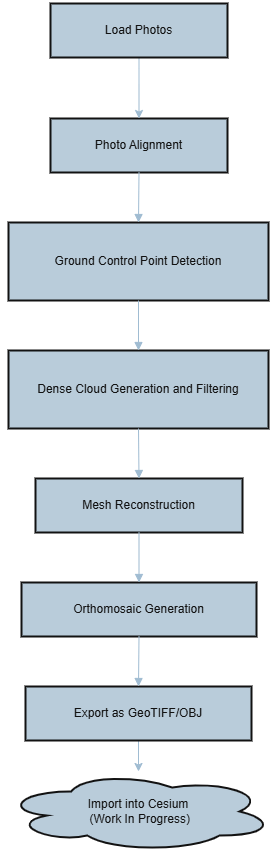
\includegraphics[width=5cm]{Images/Figures/PhotogrammetryProcessingLT.png}
    \caption{Flow chart of Photomosaic data flow in Metashape}
    \label{fig:photogrammetry_flow}
\end{figure}

In Agisoft Metashape, the photogrammetry workflow starts by \textbf{aligning} photos to find matching points and build a sparse 3D cloud that defines how the images fit together. \textbf{Ground control points} (GCPs) are then imported. The GCPs are the steel markers placed around the survey area and the QR codes are automatically detected by metashape before alignment.

From there, a \textbf{dense cloud} is generated to capture detailed surface geometry, and low-confidence points are filtered out to keep the data clean.

The next step is mesh \textbf{reconstruction}, which connects those points into a continuous 3D. Once the geometry is complete, Metashape projects the photos onto it, producing a georeferenced orthomosaic that accurately represents the site. Finally, the results are exported.

\subsubsection{Scripting}

\tcbset{colback=gray!5,colframe=gray!40,boxrule=0.5pt,sharp corners,enhanced}

\begin{tcolorbox}[title=Add Photos]
\texttt{chunk.addPhotos(image\_list)} --- Loads all images from A..Z folders.
\end{tcolorbox}

\begin{tcolorbox}[title=Photo Alignment]
\texttt{chunk.matchPhotos(...)} then \texttt{chunk.alignCameras()} --- Finds matching features across images.
\end{tcolorbox}

\begin{tcolorbox}[title=GCP Import \& Optimization (if used)]
\texttt{chunk.importReference(...)} and \texttt{chunk.optimizeCameras(...)} --- Brings in control points and refines the alignment so the model is accurately scaled/georeferenced.
\end{tcolorbox}

\begin{tcolorbox}[title=Dense Cloud Generation \& Filtering]
\texttt{chunk.buildDepthMaps(downscale=..., filter\_mode=...)} --- Computes depth for each image to create dense geometry.
\end{tcolorbox}

\begin{tcolorbox}[title=Mesh Reconstruction]
\texttt{chunk.buildModel(source\_data=Metashape.DepthMapsData, surface\_type=Metashape.Arbitrary)} --- Converts dense depth information into a continuous 3D surface (mesh).
\end{tcolorbox}

\begin{tcolorbox}[title=Orthomosaic Generation]
\texttt{chunk.buildOrthomosaic(surface=Metashape.ModelData, ...)} --- Projects the photos onto the mesh and blends the mosaic image.
\end{tcolorbox}

\begin{tcolorbox}[title=Export as GeoTIFF/OBJ]
\texttt{chunk.exportOrthomosaic(ORTHO\_OUT, image\_format=TIFF, ...)} --- Writes the orthomosaic to disk.
\end{tcolorbox}

The following is a link to the Metashape Python API:
\href{https://www.agisoft.com/pdf/metashape_python_api_2_2_0.pdf}{link}.
% \cite{agisoft_metashape_api_2024} % keep if you already have this bib entry

\newpage
\subsection{In Summary}
I’m organizing my underwater photos to track completed locations and outline the photomosaic workflow. Using the Metashape GUI for each dataset can be slow and repetitive. Agisoft Metashape offers a Python API that I can integrate into my project pipeline. As I begin incorporating larger datasets from online sources, this will help automate the photomosaic creation process and reduce manual work through the GUI.

\newpage

% ===============================
% Bibliography
% ===============================
\bibliographystyle{plain}
\bibliography{references}

\end{document}
